
We know that the point $(X,Y)$ satisfies the equation 
\begin{align}
x^2 + y^2 \leq r^2 
\end{align}
Let a random variable $Z\in \{0,1\}$ denote the possible outcomes of the experiment
\begin{table}[h]
\centering
    \begin{tabular}{|c|c|}
        \hline
        Equation satisfied by (X,Y)& Z    \\\hline
        $y-mx<0$ & 0    \\\hline
        $y-mx\geq0$ & 1 \\\hline
    \end{tabular}
\caption{Outcome of the Experiment}
\label{ma2001-2.23:table=1}
\end{table}

The coordinates $(X,Y)$ can be parametrized as follows:
\begin{align}
    X = a\sin\theta\\
    Y = a\cos\theta
\end{align} 
where $a \in [0,r]$ and $\theta \in [0, 2\pi]$. 
\begin{align}
    Y &\geq mX\\
    \implies a\sin\theta &\geq ma\cos\theta
\end{align}

\begin{figure}[h]
    \centering
    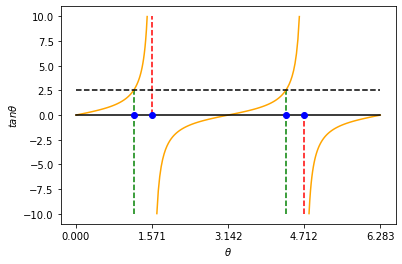
\includegraphics[width=\columnwidth]{solutions/adv/ma/2001/2.23/figures/tanx.png}
    \caption{$tan\theta$ with $m=2.5$}
    \label{ma2001-2.23:tanx}
\end{figure}

This gives two cases for an arbitrary value of $m$ (as seen in fig \ref{ma2001-2.23:tanx}):
\begin{enumerate}
    \item when $\theta\in \left[0,\dfrac{\pi}{2}\right]\cup\left[\dfrac{3\pi}{2},2\pi\right]$, from \ref{ma2001-2.23:tanx},
    \begin{align}
        \tan\theta&\geq m\\
        \implies \theta &\in [\tan^{-1}m, \pi/2]
    \end{align}
    \item similarly, when $\theta \in \left[\dfrac{\pi}{2}, \dfrac{3\pi}{2}\right]$
    \begin{align}
        \tan\theta&\leq m\\
        \implies \theta &\in [\pi/2, \pi+\tan^{-1}m]
    \end{align}
\end{enumerate}
\begin{align}
    \therefore \theta &\in [\tan^{-1} m, \pi+\tan^{-1} m]
\end{align}

$\theta$ will have a uniform probability distribution function: 
\begin{align}
    f(\theta)=\nonumber
    \begin{cases}
    0 &\text{if } \theta<0\\
    \dfrac{1}{2\pi} & \text{if } 0\leq\theta\leq2\pi\\
    0 &\text{if } \theta>2\pi
    \end{cases}
\end{align}
The shaded region of figure \ref{ma2001-2.23:fig:my_label} represents the required probability. 
\begin{align}
    \pr{\arctan m\leq\theta\leq\tan^{-1} m +\pi}\nonumber\\
    =\displaystyle\int\limits_{\tan^{-1} m}^{\pi + \tan^{-1} m} f(\theta) \,d\theta
\end{align}
\begin{align}
    &=\displaystyle\int\limits_{\tan^{-1} m}^{\pi + \tan^{-1} m} \frac{1}{2\pi} \,d\theta\\
    &=\frac{\pi}{2\pi}\\
    &=\frac{1}{2}
\end{align}
\begin{figure}[h!]
    \centering
    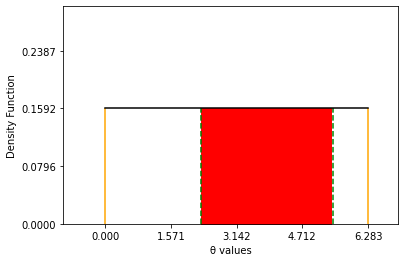
\includegraphics[width=\columnwidth]{solutions/adv/ma/2001/2.23/figures/distribution_2.png}
    \caption{Distribution function of $\theta$}
    \label{ma2001-2.23:fig:my_label}
\end{figure}\\
\\ $\therefore$ option (c) is correct.


